%RC, RL circuits for sample questions, also some sinusoidal waves

\documentclass{article}

\usepackage{tikz}
\usepackage{circuitikz}
\usepackage{tkz-euclide}
\usepackage{pgfplots}
\usetikzlibrary{arrows.meta}

\begin{document}

\begin{center}
\begin{circuitikz}
\draw (0,0)
to[battery, l=$5\, V$] (0,2)
to[short] (1.5,2)
to[R=$100\, \Omega$] (2.5,2);
\draw (2.5,2)
to[short] (4,2)
to[C=$4\, \mu F$] (4,0)
to[short] (0,0);
\end{circuitikz}
\\{RC circuit of Q2}
\end{center}

\begin{center}
\begin{circuitikz}
\draw (0,0)
to[battery, l=$4.5\, V$] (0,2)
to[short] (1.5,2)
to[R=$20\, \Omega$] (2.5,2);
\draw (2.5,2)
to[short] (4,2)
to[L=$1\, mH$] (4,0)
to[short] (0,0);
\end{circuitikz}
\\{RL circuit of Q3}
\end{center}

\begin{center}
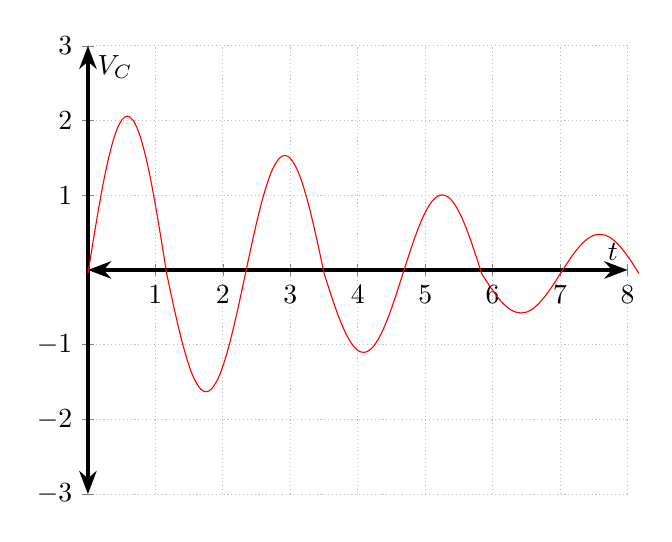
\begin{tikzpicture}
\begin{axis}[
  axis lines=middle,
  axis line style={Stealth-Stealth,very thick},
  xmin=0,xmax=8, ymin=-3,ymax=3,
  xtick distance=1,
  ytick distance=1,
  xlabel=$t$,
  ylabel=$V_C$,
  grid=major,
  grid style={thin,densely dotted}]
\end{axis}
\draw[red] (0,2.8) sin (0.5,4.8) cos (1,2.8) sin (1.5,1.3) cos (2,2.8) sin (2.5,4.3) cos (3,2.8) sin (3.5,1.8) cos (4,2.8) sin (4.5,3.8) cos (5,2.8) sin (5.5,2.3) cos (6,2.8) sin (6.5,3.3) cos (7,2.8);
\end{tikzpicture}
\\{Example Plot for $V_C$ wrt t}
\end{center}
\bigskip

\begin{center}
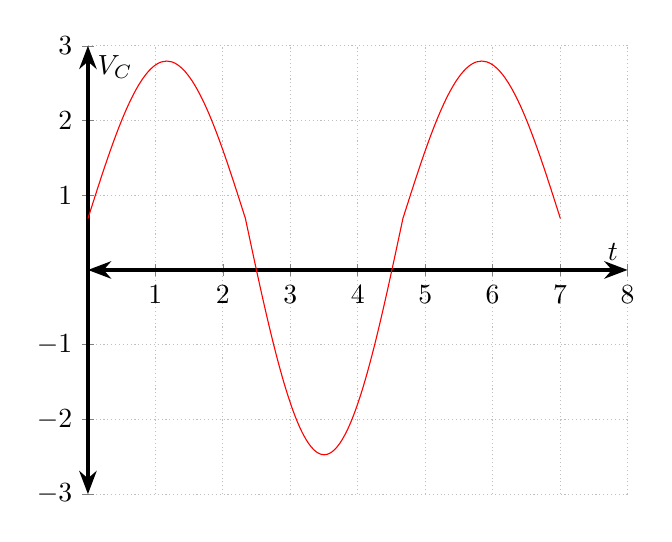
\begin{tikzpicture}
\begin{axis}[
  axis lines=middle,
  axis line style={Stealth-Stealth,very thick},
  xmin=0,xmax=8, ymin=-3,ymax=3,
  xtick distance=1,
  ytick distance=1,
  xlabel=$t$,
  ylabel=$V_C$,
  grid=major,
  grid style={thin,densely dotted}]
\end{axis}
\draw[red] (0,3.5) sin (1,5.5) cos (2,3.5) sin (3,0.5) cos (4,3.5) sin (5,5.5) cos (6,3.5);
\end{tikzpicture}
\\{Example Plot for $V_C$ wrt t}
\end{center}

\end{document}
